% \chapter{Introduction}
% \label{introduction}


% \begin{itemize}
    %     \item Chiral review \cite{epelbaum_frontiers}
    
    %     \item Weinberg \cite{WEINBERG1990}\\
    %         Weinberg \cite{WEINBERG1990} suggested using a most general Lagrangian
    %         satisfying spontaneously broken chiral symmetry and other symmetries and
    %         evolving pions together with low-energy nucleons.
    
    %         \item Epelbaum \cite{epelglockle98, epelglockle2000, epelglockle2003}
    %     \item The newest chiral force \cite{reinkrebs2018} 
    
    %     \item Arenhovel \cite{ArenhovelPhotodisint1991}
    %     \begin{itemize}
        %         \item He used different currents (`names, types')
        %         \item Approaches
        %     \end{itemize}
        % \end{itemize}
% \section{Historical overview}
        
% In the second half of XX century physical society faced
% a problem of describing low-energetic nuclear reactions.
% \gls*{qcd} is hardly applicable here as it is nonperturbative 
% at low energies what complicates a lot search for the solutions \cite{Machleidt2011}. 


% \printglossary[type=\acronymtype]
% \printnoidxglossary[type=acronym]

\chapter{Plan}

\begin{itemize}
    \item Why we study few nucleon systems
    \begin{itemize}
        \item Strong interactions (2N and 3N force investigation; QCD, relativistic effects)
        \item Electro-magnetic processes (electrons-, photons-induced reactions) (Arenhovel did ...)
        \item Weak interactions (neutrons)
    \end{itemize}

    \item Nuclear forces used in the thesis
    \begin{itemize}
        \item AV18
        \item Chiral (scs, sms; difference between chiral models; regularization problem)
    \end{itemize}

    \item Currents used in the thesis (regularization of currents to be done)
    
    \item Formalism \& numerical methods
    \begin{itemize}
        \item Lippman-Schwinger eq
        \item Schrodinger eq for deuteron; wave functions (sms) for deuteron - figures, binding energy
        \item Three body: Fadeev eq. for bound (He3, H3) and scattering states
        \item Siegert theorem ?
        \item Partial wave decomposition, states ($pq\alpha$), Jakobi momenta;
        operators in PW decomp. (current); Mathematica for PW
        \item Theoretical uncertainties: truncation error, cut-off dependency, chiral order dependency
    \end{itemize}

    \item Results (\textbf{find everything what I have calculated: all processes and energies} )
    \begin{itemize}
        \item H2 photodisintegration
        \item He3 and H3 photodisintegration
        \item Pion capture
    \end{itemize}

    \item Summary
    
    \item References
\end{itemize}

\subsection*{Why we study few nucleon systems}

The study of light nuclei for the decades has been serving as an easiest way
to study NN systems and forces inside the atom. And
convenient way to proceed may be an interaction of atom with
other particles: elastic or inelastic scattering.
It is possible to construct such an experiments and check if theory works.
People take into account that interactions may be caused by different forces
and therefore should be described in different ways. It can be
either strong, weak or electromagnetic interaction. It depends
on the type of particle being scattered and the target which reaction it is.

In order to proper describe the nuclear reactions many
factors should be taken into account.
First of all, different nuclear forces may act on
the participants.


The strong nuclear force appear inside the nuclei and among others bound neutrons 
and protons together. The description of strong interactions is extremely
difficult as it deals not only with nucleon, but with their constituents: quarks
and gluons. Quantum Chromodynamics(QCD) is a modern theory
describing strong interactions, but it has also its limitations at the moment
as it is not reliable at low energies ($Q^2 \lesssim 1 GeV^2$).
So other approaches are coming into the scene such as 
chiral effective theory, lattice calculation and others \cite{IOFFE2006232}.

Electromagnetic force appears between charged particles like protons and electrons.
Also, the force is transferred between charged particles with a photon, so 
in photon- and electron- scatterings on the nuclei an electromagnetic
force is playing an important role. Arenhovel \cite{ArenhovelPhotodisint1991} 
studied electromagnetic process - Deuteron photodisintegration,
applying different approaches and comparing the results with
experimental data.

The weak force...

...  

Starting the study of 3- (and more) nucleon systems it was found that 2N force is not enough to describe
the system and 3N force was introduced. The first applications of such
a force showed that it brings sufficient contribution and cannot be ignored \cite{GLOCKLE1982343}.
Whereas the first applications included only early "realistic" potential, the latter
investigations only proved this statements \cite{StoksPhysRevC49, WIRINGAPhysRevC51}.
It was also used to construct four-nucleon (4N) bound state \cite{NoggaPhysRevLett}.

...
\subsection*{Nuclear forces used in the thesis}

In order to construct a potential people often use phenomenological
or semi-phenomenological approaches. It allows to combine
theoretical knowledge about processes and experimental data.

One of such potentials, which was used in current thesis is Argonne V18 (AV18) \cite{AV18Wiringa} 
In order to construct NN force, authors combine
analytical electromagnetic and one-pion-exchange parts
with phenomenological one, fitting parameters to
the Nijmegen partial-wave analysis of $pp$ and $np$ data \cite{NijmegenPhysRevC.48.792}. 
Authors showed, that AV18 potential delivers good results
in the description of nucleon scattering data as well as deuteron 
properties. 


In the early 1990-ies Weinberg \cite{WEINBERG1990,WEINBERG1991} introduced 
an idea of using a most general Lagrangian
satisfying assumed symmetry principles and in particular
spontaneously broken chiral symmetry to 
describe nuclear interactions at low energies.
This idea together with \gls*{eft} of \gls*{qcd} 
led to the development of \gls*{ceft}
% a Chiral effective field theory ($\chi$EFT)
which nowadays has become one of the most advanced approach to
describing nuclear reactions at low energies.
 
For the \gls*{eft} it is very important to 
define a quantity, which powers will determine a perturbation order.
In the \gls*{ceft} there are two natural scales: so-called soft scale -
the mass of Pion $Q \sim M_\pi$ and hard scale -
$\Lambda_\chi \sim 1~GeV$ (chiral symmetry breaking scale).
The ratio between these two scales $(Q/\Lambda_\chi)^\nu$
is being used as an expansion parameter in  \gls*{ceft} with power
$\nu$.

Considering so-called irreducible (the diagrams that cannot be split
by cutting nucleon lines), Weinberg \cite{WEINBERG1990,WEINBERG1991}
came to the identity for the powers of such diagrams\cite{Machleidt2011}:

\begin{equation}
    \nu_W = 4 - A - 2C + 2L + \sum_i \Delta_i,
    \label{powers}
\end{equation}
where

\begin{equation}
    \Delta_i \equiv d_i + \frac{n_i}{2} - 2
    \label{Delta}
\end{equation}

In \ref*{powers}, $C$ is a number of pieces which are connected, $L$ - the number of loops in the graph.
In \ref*{Delta}, $n_i$ is a number of nucleon field operators, $d_i$ - the number of insertions
(or derivatives) of  $M_\pi$.

In \gls*{ceft} the first order is called "leading order" (LO)  and it is followed 
by next-to-leading order (NLO), next-to-next-to-leading order (N2LO) and so on.
At the moment, the highest order for which there is a derived term in potential
is N4LO. Also some contributions from N5LO are included in the N4LO+ chiral order. 


As pointed above, for many-nucleon systems it is important to include not 
only nucleon-nucleon interaction to the potential, but also a 3- and many- nucleon
contributions. In the \gls*{ceft} 3N force contributes starting from N2LO and
4N force is presented starting from N3LO, so there is a systematic
way to include all the forces from simplest diagrams at LO and gradually
adding more and more terms. It is also beneficial in the way that 
one can obtain results using chiral potential at different
orders and track which one gives larger or smaller contribution (changes in the
final results).

The \gls*{ceft} may be applied both in coordinate and momentum spaces.
Nevertheless in both cases it requires regularization which is cutting 
low coordinate values in order to avoid infinities 
(or high momentum values - in momentum space). 
The SMS potential is being regularized using the Gaussian form factor
$F(\vec{l}^2)$:

\begin{equation}
    F(\vec{l}^2) = e^{-\frac{\vec{l}^2 + M_\pi^2}{\Lambda^2}},
    \label{regulator}
\end{equation}
where $M_\pi$ is an effective pion mass and $\Lambda$ - is a cutoff parameter.

The form factor from \eq{regulator}, being used together with Feynman propagator,
ensures that long-range part of the forces has no singularities. 

The value at which
the cut is applied (cut-off value) is not fixed and usually calculations
are being performed for different cut-off values. The comparison
of such results may reveal stronger or weaker dependance and in perfect
case one will come up with such a potential, were the cut will
not affect results much. On the Fif.~\ref{potential_cutoff} 
I show values of the 2N potential $\matrixel{\vec{p}}{V}{\pvec{p}}$
as a function on the momentum $|\vec{p}|$ with fixed value $|\pvec{p}|$=0.054[fm].



\begin{figure}[htb]
    \begin{center}
    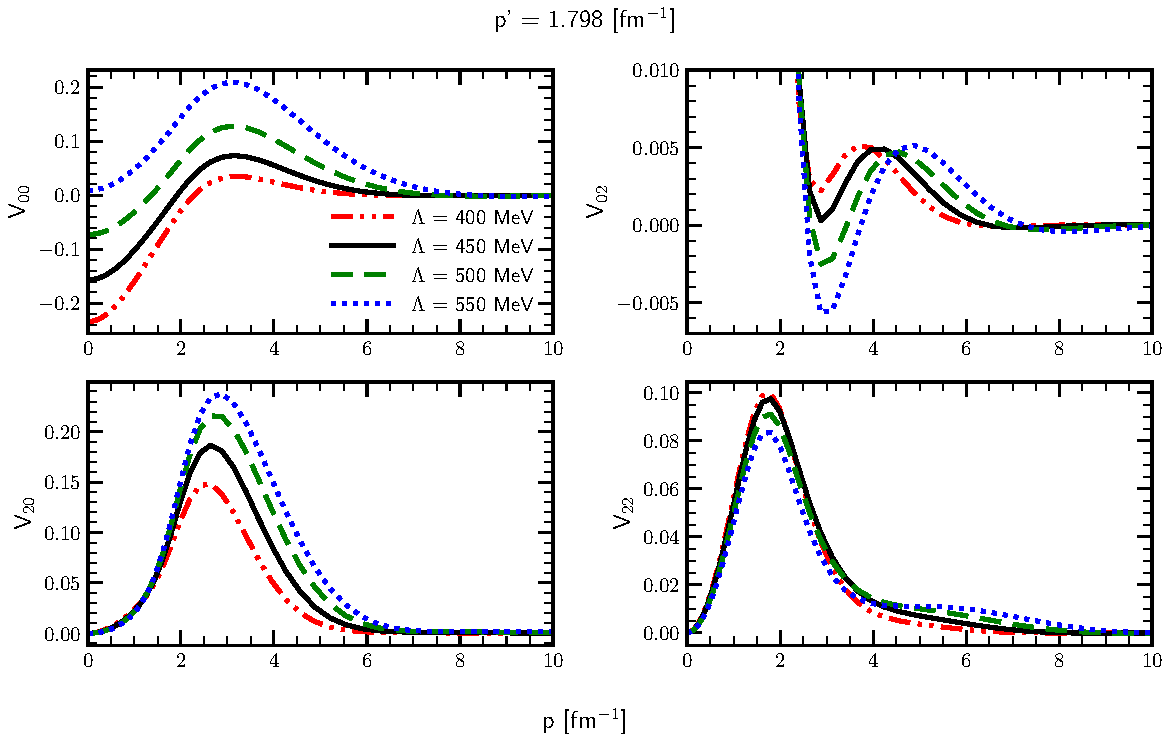
\includegraphics[width=0.95\textwidth]{PlotData/Deuteron/WAVEFUNC/potential_pp1.798.pdf}
    \end{center}
    \caption{Potential components as a function on the momentum $p$ with fixed
    value of the momentum $p'$=1.798 [fm?].
    }
    \label{potential_cutoff}
\end{figure}



The potential may be transformed from coordinate to momentum space (or vice versa),
but it is important at which frame the regularization was performed
and what was a regularization function. That's why there are different 
versions of chiral potential. One is semi-local coordinate space regularized potential (SCS) \cite{Epelbaum2014SCS}
and another one is similar, but with regularization applied in momentum space (SMS potential) \cite{reinkrebs2018}.


\subsection*{Currents}
 
% When it comes to the study of scattering processes on nuclei one has 
% to construct nuclear matrix elements, the crucial part 
% of which is nuclear current. The currents should be consistent with
% the force used

